\documentclass[xcolor=dvipsnames]{beamer}

% font setup
\usepackage{libertine}
\renewcommand*\familydefault{\sfdefault}    % Linux Libertine = default sans serif
\usepackage{inconsolata}                    % Inconsolata = monospaced
\usepackage[utf8]{inputenc}
\usepackage[T1]{fontenc}

% Graphics and other packages
\usepackage[romanian]{babel}
\usepackage{graphicx}
\addto\captionsromanian{\renewcommand{\figurename}{Ilustrație}}
\usepackage{caption}
\usepackage{subcaption}
\usepackage[style=german]{csquotes}

% Custom macros
\newcommand{\bloc}[3]{\begin{bl}<#1->{{\large\color{Gray}{\hrulefill}}\\ \color{bleumarin}{\large \emph{#2}}}\\ \vspace*{-2mm}{\color{Gray}{\hrulefill}}\\ #3 \end{bl}} 
\newcommand{\fr}[1]{\frame{#1}}
\newcommand{\ft}[1]{\frametitle{\color{bleumarin}{\hfill #1 \hfill}}}
\newcommand{\lin}[3]{\uncover<#1->{\alert<#1>{#2}}{\vspace*{#3 ex}}}
\newcommand{\ite}[2]{\uncover<#1->{\alert<#1>{\item #2}}}
\newcommand{\vs}[1]{\vspace*{#1 ex}}
\definecolor{bleumarin}{RGB}{30,30,150} 
\definecolor{firebrick}{RGB}{178,34,34}

% Theme setup
\useoutertheme{shadow} 
\usetheme{CambridgeUS} 
\usecolortheme[named=bleumarin]{structure} 
\useoutertheme[compress]{smoothbars}

% Theme finetuning
\setbeamertemplate{items}[ball]
\setbeamertemplate{blocks}[rounded][shadow=true]
\setbeamertemplate{navigation symbols}{}
\setbeamertemplate{headline}{}  


%%%%%%%%%%%%%%%%%%%%%%%%%%%%%%%%%%%%%%%%%%%%%%%%%%%%%%%%%%%%%%%%%%%%%%
% TITLE PAGE
\title[Tor]{The Onion Router (Tor)}
\author[Bucurescu, Manea, Nicolae]{Cornel Bucurescu, Adrian Manea, Cristian Nicolae}
\institute[SecRet]{SLA, 406 \& 410}

\date{}

\begin{document}

\maketitle
%%%%%%%%%%%%%%%%%%%%%%%%%%%%%%%%%%%%%%%%%%%%%%%%%%%%%%%%%%%%%%%%%%%%%%


% SLIDES START HERE
%%%%%%%%%%%%%%%%%%%%%%%%%%%%%%%%%%%%%%%%%%%%%%%%%%%%%%%%%%%%%%%%%%%%%%
\fr{                            % begin frame (custom macro [see preamble])
  \ft{Ideea principală (TL;DR)}             % \frame title (custom macro [see preamble])
  \begin{figure}[!htbp]
    \centering
    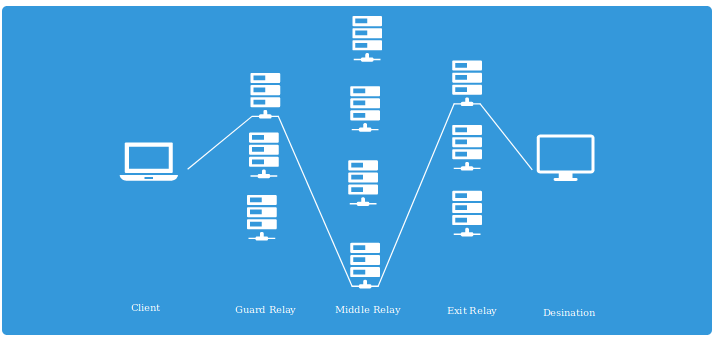
\includegraphics[scale=0.45]{../latex/fig/3relays.png}
    \caption{Cele 3 relee dintr-o conexiune standard \cite{jw1}}
  \end{figure}
}
%%%%%%%%%%%%%%%%%%%%%%%%%%%%%%%%%%%%%%%%%%%%%%%%%%%%%%%%%%%%%%%%%%%%%%

\fr{
  \ft{Ideea principală (TL;DR)}
  \begin{figure}[!htbp]
    \centering
    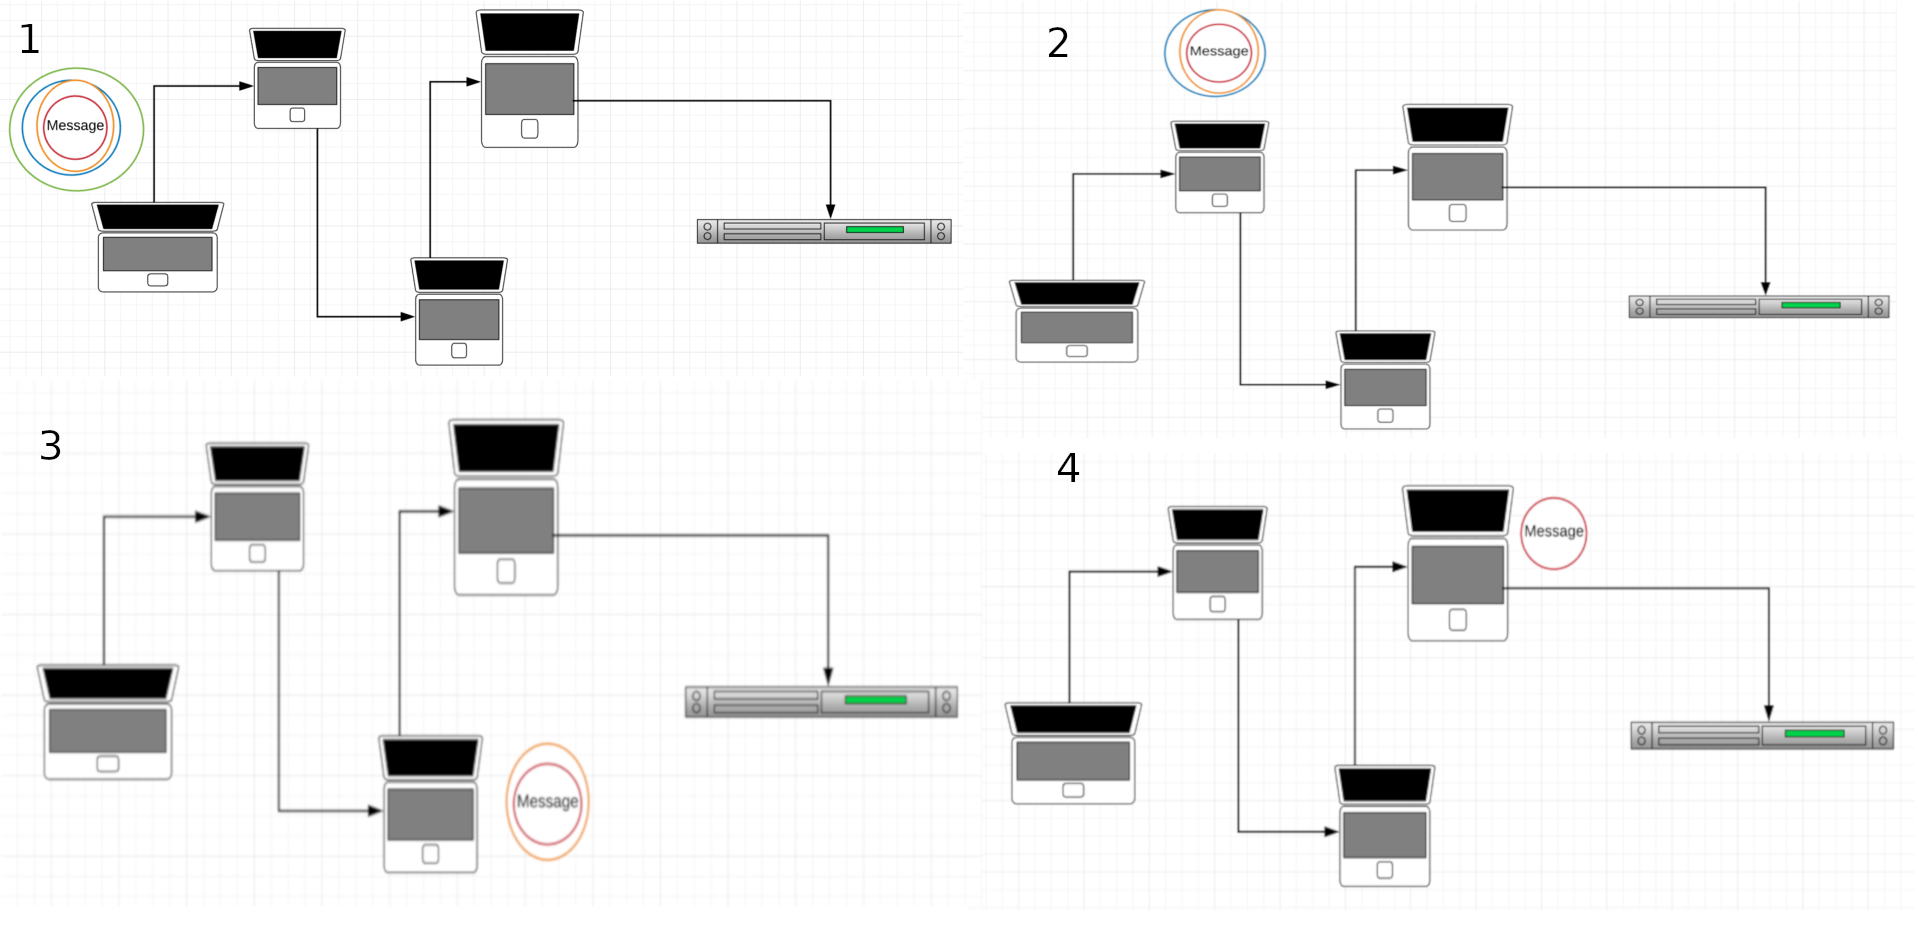
\includegraphics[scale=0.7]{../latex/fig/4onions.png}
    \caption{Criptarea telescopică \cite{bs}}
  \end{figure}
}
%%%%%%%%%%%%%%%%%%%%%%%%%%%%%%%%%%%%%%%%%%%%%%%%%%%%%%%%%%%%%%%%%%%%%%

\fr{
  \ft{Obiective de design (2004)}
  \begin{itemize}
    \ite{1}{perfect forward secrecy;}
    \ite{2}{separarea filtrării de anonimitate;}
    \ite{3}{TCP streams multiplexing;}
    \ite{4}{topologie ``leaky pipe'';}
    \ite{5}{autorități directoare;}
    \ite{6}{servicii ascunse.}
\end{itemize}
}
%%%%%%%%%%%%%%%%%%%%%%%%%%%%%%%%%%%%%%%%%%%%%%%%%%%%%%%%%%%%%%%%%%%%%%

\fr{
  \ft{Non-obiective (limitări admise)}
  \begin{itemize}
    \ite{1}{nu servește drept conexiune peer-to-peer (vulnerabilă!);}
    \ite{2}{nu protejează împotriva atacurilor end-to-end (timing, intersection);}
    \ite{3}{nu normalizează protocoalele;}
    \ite{4}{nu ascunde traficul ($ \neq $ \emph{steganografic}).}
\end{itemize}
}
%%%%%%%%%%%%%%%%%%%%%%%%%%%%%%%%%%%%%%%%%%%%%%%%%%%%%%%%%%%%%%%%%%%%%%

\fr{
  \ft{Funcționare}

  \lin{1}{Modelul este de ``overlay network''.}{2}

  \lin{2}{OR au chei de identitate (IDK) și cheie onion (OK).}{2}

  \lin{3}{IDK semnează certificate TLS și directoarele.}{2}

  \lin{4}{OK decriptează cererile, stabilește circuite și negociază cheile efemere.}{2}

  \lin{5}{Comunicarea se face prin TLS cu chei efemere.}{2}

  \lin{6}{Traficul circulă în \emph{celule de cîte 512 bytes}, cu \emph{header} și \emph{payload}.}{2}
}
%%%%%%%%%%%%%%%%%%%%%%%%%%%%%%%%%%%%%%%%%%%%%%%%%%%%%%%%%%%%%%%%%%%%%%

\fr{
  \ft{Construcția unui circuit Alice $\longrightarrow$ Bob}

  \lin{1}{Alice $\xrightarrow{\texttt{create}}$ Bob și alege \texttt{circID} $C_{AB}$.}{2}

  \lin{2}{Alice $\xrightarrow{\texttt{OK} = g^x}$ Bob.}{2}

  \lin{3}{Bob $\xrightarrow{\texttt{created} = g^y, \quad hash(K = g^{xy})}$ Alice.}{2}

  \lin{4}{Acum, Alice și Bob pot comunica folosind cheia $ K $.}{2}
}
%%%%%%%%%%%%%%%%%%%%%%%%%%%%%%%%%%%%%%%%%%%%%%%%%%%%%%%%%%%%%%%%%%%%%%

\fr{
  \ft{Extinderea circuitului Alice $ \to $ Bob $ \to $ Carol}

  \lin{1}{A $\xrightarrow{\texttt{relay extend}, \quad g^{x_2}, \quad \texttt{addr(C)}} $ Bob.}{2}

  \lin{2}{Bob $ \xrightarrow{\texttt{create}} $ Carol \&\& copy($g^{x_2}$) \&\& alege \texttt{circID} $C_{BC}$.}{2}

  \lin{3}{Carol $\xrightarrow{\texttt{created} = g^{y_2}} $ Bob $\xrightarrow{\texttt{payload}}$ Carol.}{2}

  \lin{4}{Bob $ \xrightarrow{\texttt{relay extended}} $ Alice.}{2}

  \lin{5}{Acum, se poate comunica A---C cu cheia $ K_2 = g^{x_2y_2} $.}{2}
}
%%%%%%%%%%%%%%%%%%%%%%%%%%%%%%%%%%%%%%%%%%%%%%%%%%%%%%%%%%%%%%%%%%%%%%

\fr{
  \ft{Circuit cu 3 relee}

  \begin{figure}[!htbp]
    \centering
    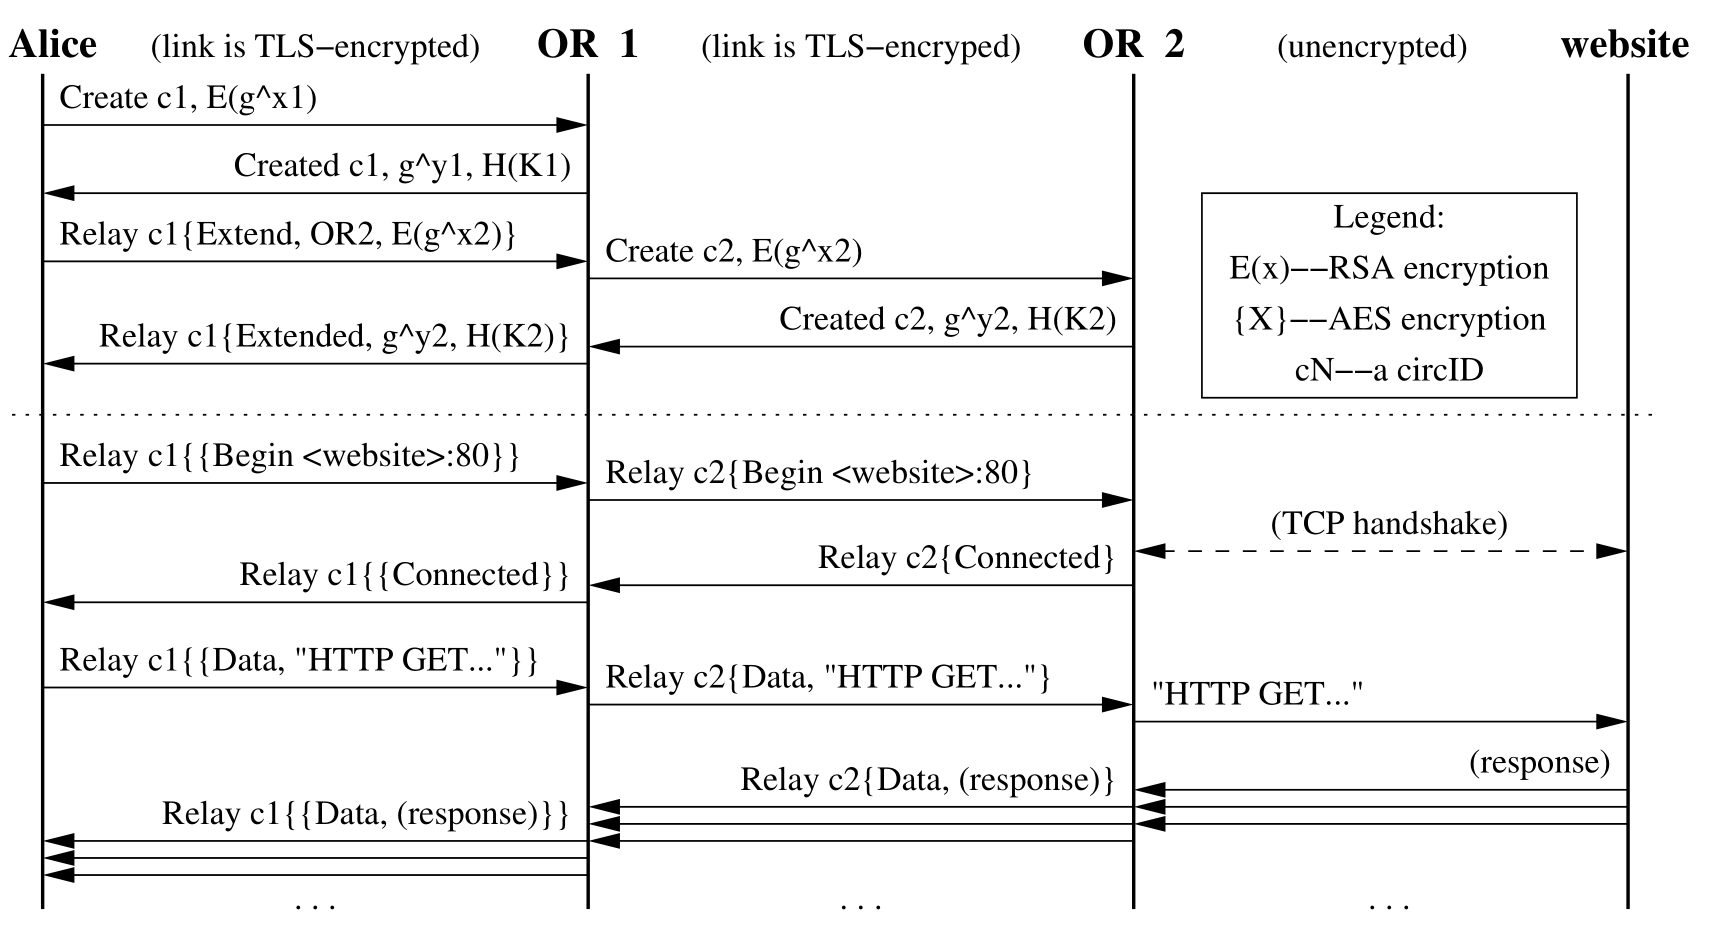
\includegraphics[scale=0.8]{../latex/fig/cells.png}
    \caption{Celule schimbate la inițierea unui circuit (\cite{whitepaper}, \S4.1}
  \end{figure}
}
%%%%%%%%%%%%%%%%%%%%%%%%%%%%%%%%%%%%%%%%%%%%%%%%%%%%%%%%%%%%%%%%%%%%%%

\fr{
  \ft{Servicii ascunse (\texttt{[hash].onion})}

  \lin{1}{Serverul ascuns creează o pereche de chei pentru criptare asimetrică și 
  cere unui OR să devină punct de intrare.}{2}

  \lin{2}{După acceptare, serverul pune într-un \emph{tabel de hash-uri distribuit} IP-urile
  punctelor de introducere acceptate.}{2}

  \lin{3}{Clientul primește adresa de tip \texttt{[hash].onion} (cheia publică), 
  deci știe IP-urile cu care poate intra în Tor.}{2}

  \lin{4}{Clientul creează o celulă de introducere, cu adresa nodului ales pentru acces.}{2}

  \lin{5}{Nodul decriptează celula de introducere cu cheia privată și acceptă clientul.}{2}

  \lin{6}{Comunicarea se face cu un nod intermediar, deci conexiunea cu serverul ascuns
  are cel puțin 6 noduri.}{2}
}
%%%%%%%%%%%%%%%%%%%%%%%%%%%%%%%%%%%%%%%%%%%%%%%%%%%%%%%%%%%%%%%%%%%%%%

\fr{
  \ft{Autorități directoare (AD)}
    \lin{1}{Există cîteva autorități directoare = noduri de încredere.}{0}

    \lin{2}{AD votează și actualizează statusul rețelei în \emph{consens}:}{0}
    \begin{itemize}
      \ite{3}{fac o listă de relee cunoscute;}
      \ite{4}{calculează alți parametri necesari (țara, lățimea de bandă);}
      \ite{5}{transmit cele de mai sus către celelalte AD, ca status;}
      \ite{6}{rezultă un \enquote{status mediat};}
      \ite{7}{din status $\Rightarrow$ vot, transmis între AD cu semnătură.}
  \end{itemize}

  \lin{8}{Votul și actualizarea sînt publice.}{0}
}
%%%%%%%%%%%%%%%%%%%%%%%%%%%%%%%%%%%%%%%%%%%%%%%%%%%%%%%%%%%%%%%%%%%%%%

\fr{
  \ft{{\color{firebrick}Atacuri $\times$} {\color{ForestGreen} apărări}}

  \lin{1}{\textbf{Pasive:}}{0}
  \begin{itemize}
    \ite{2}{Observarea tiparelor de trafic $\times$ {\color{ForestGreen} TCP streams multiplexing};}
    \ite{3}{End-to-end correlation $\times$ {\color{ForestGreen} leaky pipe topology};}
    \ite{4}{Confirmation attacks, website fingerprinting $\times$ {\color{ForestGreen} celule mici, padding}.}
\end{itemize}

\lin{5}{\textbf{Active:}}{0}
\begin{itemize}
  \ite{6}{OR impersonation $\times$ {\color{ForestGreen} chei efemere};}
  \ite{7}{Legal backdoors, probleme politice sau sociale $\times$ {\color{ForestGreen} ???};}
  \ite{8}{Cenzură la ieșire $\times$ {\color{ForestGreen} ???};}
  \ite{9}{Cenzură la intrare $\times$ {\color{ForestGreen} bridges}.}
  \end{itemize}
}
%%%%%%%%%%%%%%%%%%%%%%%%%%%%%%%%%%%%%%%%%%%%%%%%%%%%%%%%%%%%%%%%%%%%%%

% BIBLIOGRAFIE
\fr{
  \ft{Citări}
  \bibliography{torp.bib}
  \bibliographystyle{apalike}
  \nocite{*}
}
\end{document}

